%%%%%%%%%%%%%%%%%%%%%%%%%%%%%%%%%%%%%%%%%%%%%%%%%%%%%%%%%%%%%%%%%%%%%%%%
\chapter{Data} \label{chap:Data}
%%%%%%%%%%%%%%%%%%%%%%%%%%%%%%%%%%%%%%%%%%%%%%%%%%%%%%%%%%%%%%%%%%%%%%%%
\vspace{1cm}

In this study, data from two datasets were employed: Kispi---comprising two subcohorts, Kispi-mial and Kispi-irtk---and dHCP. While details are provided in the respective sections, an overview is presented in Tab.\,\ref{tab:datasets}.
\begin{table}[htbp]
    \centering
    \begin{tabular}{c|c|c|c|c|c|c}
        \toprule
        \textbf{Name} & $\textbf{N}_\textbf{n}$\textbf{/}$\textbf{N}_\textbf{p}$ & \makecell{\textbf{GA range} \\ \textbf{(weeks)}} & \makecell{\textbf{Field} \\ \textbf{strength}} & \textbf{Scanner} & \textbf{SRR} & \textbf{Parcel.} \\
        \midrule
        Kispi-mial & 15/25 & 20.0--32.8 & 1.5/3\,T* & \makecell{GE Signa \\ Discovery \\ MR450/750*} & \makecell{\textsc{mialsrtk} \\ \cite{Tourbier2015}} & 7 labels \\ \hline
        Kispi-irtk & 16/24 & 20.01--34.8 & 1.5/3\,T* & \makecell{GE Signa \\ Discovery \\ MR450/750*} & \makecell{\textsc{irtk} \\ \cite{Kuklisova2012}} & 7 labels \\ \hline
        dHCP & 267/0 & 20.9--38.3 & 3\,T & \makecell{Philips \\ Achieva} & \makecell{Cordero- \\ Grande\,\cite{CorderoGrande2018}} & 17 labels \\
        \bottomrule
    \end{tabular}
    \caption{Dataset properties. $\text{N}_\text{n}$ and $\text{N}_\text{p}$ respectively indicates the number of neurotypical and pathological cases. *The field strengths respectively refer to the scanners.}
    \label{tab:datasets}
\end{table}

\section{Kispi}
The Kispi dataset\,\cite{Payette2021, FeTA_MICCAI} originates from the University Children's Hospital of Zurich, Switzerland, in the context of the FeTA challenge. All data were acquired with ethics committee approval from the Canton of Zurich, and informed consent for the use of the data in research was obtained from the mothers. The dataset is open-access and fully anonymized.

The Kispi cohort comprises fetal brain MRI scans from subjects with both normal and pathological neurodevelopment. The pathological cases include a variety of congenital disorders, such as spina bifida and ventriculomegaly, reflecting a clinically relevant population\,\cite{FeTA2024_paper, Ciceri2024}. The dataset spans a gestational age (GA) range of approximately \numrange{20}{35} weeks. For the FeTA 2024 challenge, the Kispi data was partitioned into a training set of \num{80} volumes and a test set of \num{40} volumes, but only the training set is publicly available. The training partition consists of \num{31} neurotypical and \num{49} pathological cases\,\cite{FeTA2024_review}.

All imaging was performed on \qty{1.5}{\tesla} and \qty{3}{\tesla} GE Signa Discovery (MR450 and MR750) whole-body scanners. The acquisitions were conducted without the use of maternal or fetal sedation. Depending on the specific case, either an 8-channel cardiac coil or a standard body coil was employed\,\cite{FeTA2024_paper}. The acquisition details for the single volumes are not available.

The acquisition protocol consisted of T2-weighted single-shot fast spin-echo (\textsc{ssfse}) sequences acquired in the axial, coronal, and sagittal planes relative to the fetal brain. Key sequence parameters were maintained as follows\,\cite{FeTA2024_paper}:
\begin{itemize}
    \item \textbf{Repetition Time (TR):} \qtyrange[range-units = single, range-phrase = --]{2000}{3500}{\milli\second}.
    \item \textbf{Echo Time (TE):} \qty{120}{\milli\second} (minimum).
    \item \textbf{Flip Angle:} \qty{90}{\degree}.
    \item \textbf{Acquisition Resolution:} An in-plane resolution of \qtyproduct[product-units = power]{0.5 x 0.5}{\milli\meter} with a slice thickness ranging from \qtyrange[range-units = single]{3}{5}{\milli\meter} was employed.
    \item \textbf{Field of View and Matrix Size:} The FOV (\qtyrange[range-units = single, range-phrase = --]{200}{240}{\milli\meter}) and image matrix (\qty{1.5}{\tesla}: \numproduct{256 x 224}; \qty{3}{\tesla}: \numproduct{320 x 224}) were adjusted according to the GA and size of the fetus.
\end{itemize}

Prior to reconstruction, all acquired images for a given subject underwent a manual quality review to compile a stack of suitable scans, with at least one brain scan in each orientation. Each image stack was then reoriented to a standard anatomical plane, and a semi-automated method was used to generate the masks of the single labels in the fetal brain. Segmentations were then inspected and refined. Following these pre-processing steps, the data were processed using two distinct SR reconstruction pipelines, resulting in two sub-cohorts within the Kispi dataset. The parcellation distinguishes 7 labels: external cerebrospinal fluid (CSF), cortical gray matter (cGM), white matter (WM), ventricles (including cavum), cerebellum, deep gray matter (dGM), and brainstem (BS)\,\cite{FeTA2024_paper}.

\num{40} image stacks, that is, half of the available Kispi stacks, was processed using the \textsc{mial} Super-Resolution Toolkit (\textsc{mialsrtk}) pipeline\,\cite{Tourbier2015, MIALSRTK}. An example of this group of volumes---from now on referred to as the \enquote{Kispi-mial} sub-cohort---is shown in Fig.\,\ref{fig:kispi-mial_images}. The remaining \num{40} stacks were reconstructed using a pipeline based on the Image Registration Toolkit (\textsc{irtk})\,\cite{Kuklisova2012, irtk-simple}. For this sub-cohort---from now on referred to as the \enquote{Kispi-irtk}---an example is shown in Fig.\,\ref{fig:kispi-irtk_images}.

For both SRR methods the resulting 3D volumes have an isotropic resolution of \qtyproduct[product-units = power]{0.5 x 0.5 x 0.5}{\milli\metre}; scans were standardised to \numproduct{256 x 256 x 256} voxels\,\cite{FeTA2021_review}. The distributions of GA, pathology and image quality of both sub-cohorts are shown in Fig.\,\ref{fig:kispi_plots}. Even though the image quality for each volume is not provided in the open-access data---as it is only available as a plot in \cite{FeTA2024_review}---it can be noticed that Kispi-mial generally exhibits lower image quality compared to Kispi-irtk. Morover, while the image quality is equivalent between the neurotypical and the pathological sub-cohorts in Kispi-irtk, in Kispi-mial the lowest quality scans are predominantly found among the pathological cases. More details about the SR algorithms are given in Section \ref{sec:SuperResolutionReconstruction}.

\begin{figure}[hbt]
    \vspace{-5pt}
    \centering
    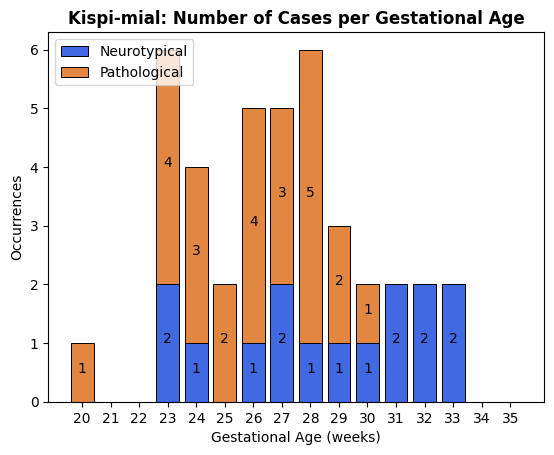
\includegraphics[width=0.45\textwidth]{figures/k-mial_GA.png} \quad
    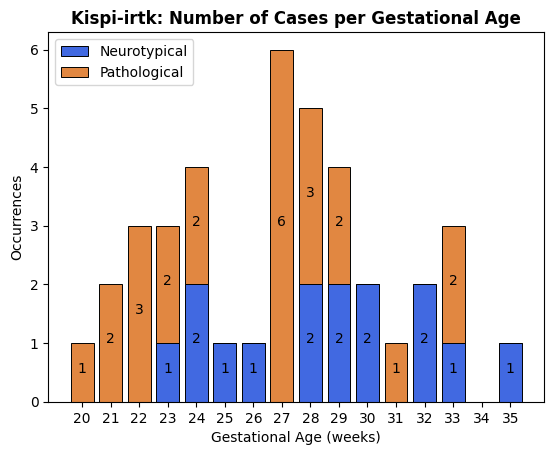
\includegraphics[width=0.45\textwidth]{figures/k-irtk_GA.png}\\
    \vspace{7pt}
    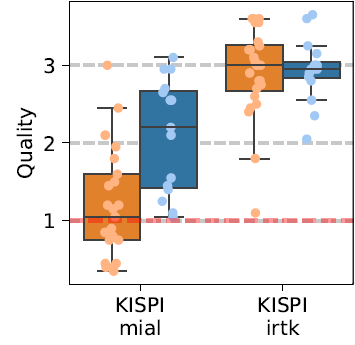
\includegraphics[width=0.32\textwidth]{figures/kispi_quality.png}
    \caption{Top: Kispi cases gestational age distribution, stratified by health condition. Bottom: Quality assessment of Kispi cases, from \cite{FeTA2024_review}.}
    \label{fig:kispi_plots}
\end{figure}

\begin{figure}[htbp]
    %\vspace{-10pt}
    \centering
    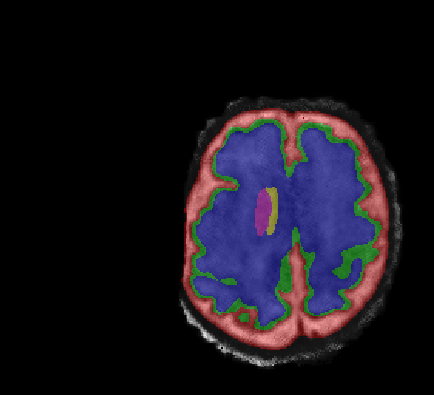
\includegraphics[width=0.33\textwidth]{figures/mial_ax_dseg.png}
    \hspace{5pt}
    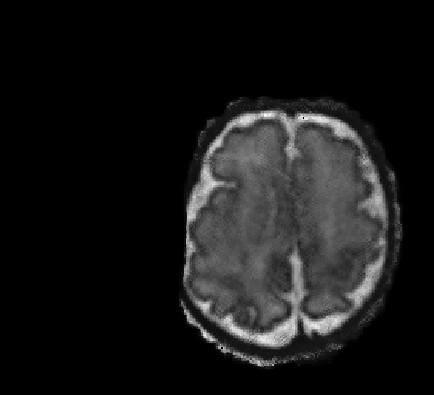
\includegraphics[width=0.33\textwidth]{figures/mial_ax.png} \\
    \vspace{10pt}
    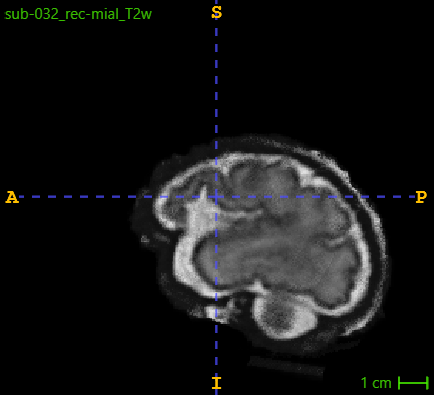
\includegraphics[width=0.33\textwidth]{figures/mial_sag.png}
    \hspace{5pt}
    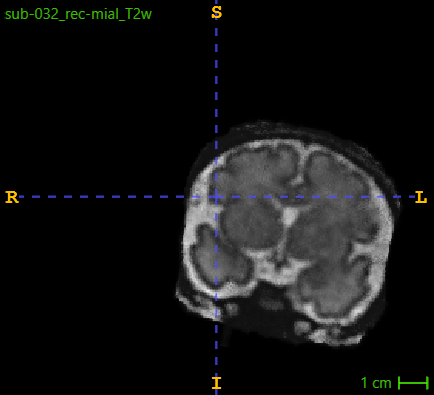
\includegraphics[width=0.33\textwidth]{figures/mial_cor.png}
    \caption{Example of Kispi-mial scan: axial segmentation, axial view, sagittal view, coronal view. Material from: \cite{Payette2021, FeTA_MICCAI}.}
    \label{fig:kispi-mial_images}
\end{figure}
\begin{figure}[htbp]
    %\vspace{-10pt}
    \centering
    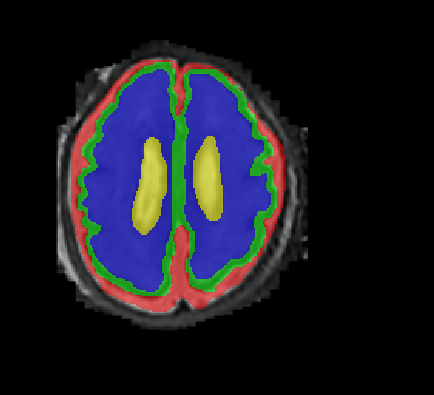
\includegraphics[width=0.33\textwidth]{figures/irtk_ax_dseg.png}
    \hspace{5pt}
    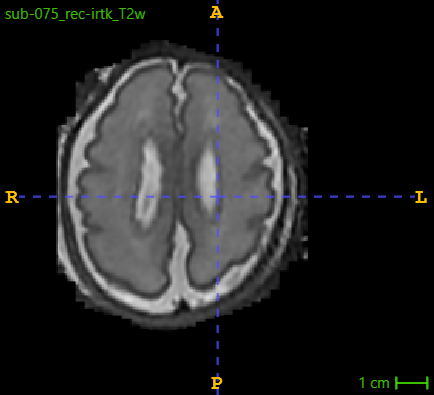
\includegraphics[width=0.33\textwidth]{figures/irtk_ax.png} \\
    \vspace{10pt}
    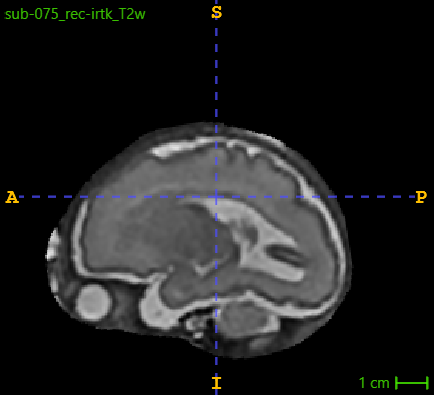
\includegraphics[width=0.33\textwidth]{figures/irtk_sag.png}
    \hspace{5pt}
    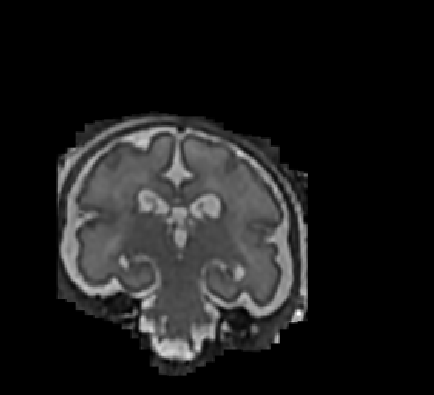
\includegraphics[width=0.33\textwidth]{figures/irtk_cor.png}
    \caption{Example of Kispi-irtk scan: axial segmentation, axial view, sagittal view, coronal view. Material from: \cite{Payette2021, FeTA_MICCAI}.}
    \label{fig:kispi-irtk_images}
    %\vspace{-5pt}
\end{figure}

\section{dHCP}
The Developing Human Connectome Project\,\cite{dHCP} (dHCP) provides an open-access spatio-temporal MRI atlas of normal fetal brain development. The dHCP fetal cohort consists of \num{296} scans from \num{272} individuals from St.\ Thomas' Hospital, London, with inclusion based on healthy pregnancies or those without major brain malformations detectable on screening ultrasound. All participants were reported by a neuroradiologist as showing age-appropriate brain anatomy on T2w anatomical scans, with no clinically significant malformations or lesions. The dataset spans a GA range from \numrange{20.86}{38.29} weeks. All imaging was performed on a Philips Achieva \qty{3}{\tesla} using a 32-channel cardiac coil. The distributions of GA and image size are shown in Fig.\,\ref{fig:dhcp_plots}. No sedation was used\,\cite{Karolis2025}.

The dHCP fetal atlas is multi-modal. For each subject, a T2-weighted anatomical scan was acquired during the same session as the functional and diffusion scans. While specific parameters for the structural sequences are not detailed---the most complete description of the fetal structural atlas is reported in an article that actually focuses on funtional MRI\,\cite{Karolis2025}---the final atlas includes T2w and T1w structural channels.

The final structural atlas was constructed from multiple 2D scans combined into high-resolution 3D volumes. Raw 2D slice data were reconstructed into isotropic 3D volumes using slice-to-volume registration (SVR), following the method illustrated in \cite{CorderoGrande2018}. The resulting volumes have a high isotropic resolution of \qtyproduct[product-units = power]{0.5 x 0.5 x 0.5}{\milli\metre}.

The atlas features a parcellation of \num{17} regions of interest, which can be merged to match exactly the 7-label scheme used in the Kispi dataset (see Tab.\,\ref{tab:label_merge} in Appendix \hyperref[app:SupplementaryTables]{B}). The segmentation is based on the dHCP structural pipeline\,\cite{Makropoulos2018, dHCP_pipeline}---an example is in Fig.\,\ref{fig:dhcp_images}. Some ground-truth segmentations are missing, bringing the number of volumes to \num{267}.

\begin{figure}[p]
    \centering
    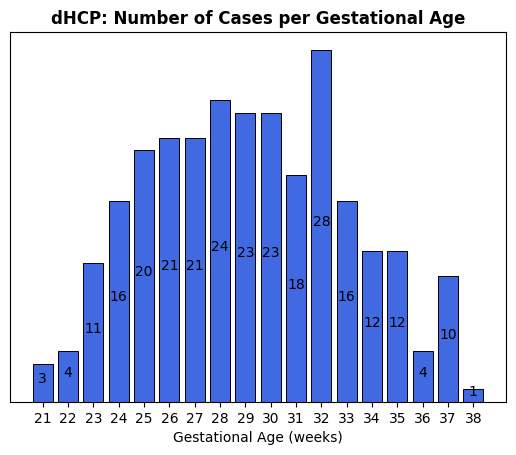
\includegraphics[width=0.47\textwidth, valign=t]{figures/dHCP_GA.png}
    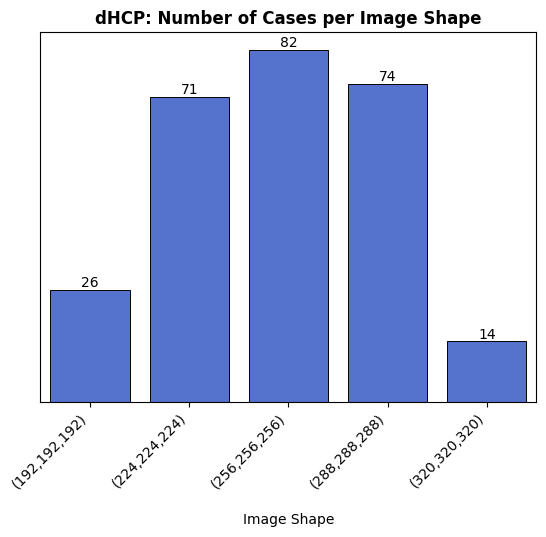
\includegraphics[width=0.5\textwidth, valign=t]{figures/dHCP_image_shape.png}
    \caption{Distributions of the gestational age and image shape of dHCP cases.}
    \label{fig:dhcp_plots}
\end{figure}
\begin{figure}[p]
    \centering
    \includegraphics[width=0.33\textwidth]{figures/dhcp_ax_dseg.png}
    \hspace{5pt}
    \includegraphics[width=0.33\textwidth]{figures/dhcp_ax.png} \\
    \vspace{10pt}
    \includegraphics[width=0.33\textwidth]{figures/dhcp_sag.png}
    \hspace{5pt}
    \includegraphics[width=0.33\textwidth]{figures/dhcp_cor.png}
    \caption{Example of dHCP scan: axial segmentation, axial view, sagittal view, coronal view. Material from: \cite{dHCP}.}
    \label{fig:dhcp_images}
\end{figure}

\section{Data Organization and File Format}

\comment{DRAFT
    The released structural dataset includes:
    \begin{itemize}
        \item T$_2$-weighted anatomical volumes (native and SVR-reconstructed).
        \item Brain masks generated by the dHCP fetal anatomical pipeline.
        \item Cortical and subcortical segmentations derived from a 3D\,U-Net-based tool\,\cite{Uus2023}.
    \end{itemize}
    All data follow the \textbf{BIDS} (Brain Imaging Data Structure) standard, with imaging files in \texttt{NIfTI} format and detailed JSON sidecar files containing acquisition metadata.
}
